
%----------------------------------------------------------------------------------------
%	Lecture 26
%----------------------------------------------------------------------------------------

\chapter{Stokes' Theorem} 

\bigbreak

\begin{mdframed}
\begin{center}
If $C$ is a closed curve then the line integral of a vector field ${\bf F}$ along $C$ can be given by
$$ \oint_{C} {\bf F} \cdot d{\bf r} = \iint_S (\nabla \times {\bf F}) \cdot \hat{n} dS $$
where $S$ can be any surface bounded by $C$ such that ${\bf F}$ is defined and differentiable everywhere on $S$.
\end{center}
\end{mdframed} 

\subsection*{Orienations} 

We need the orianations of $C$ and $S$ to be compatible.
The rule is :

If we walk along $C$ in the direction of its orientation with $S$ to the left then the normal vector is pointing up.

\begin{figure}[ht!]
    \centering
    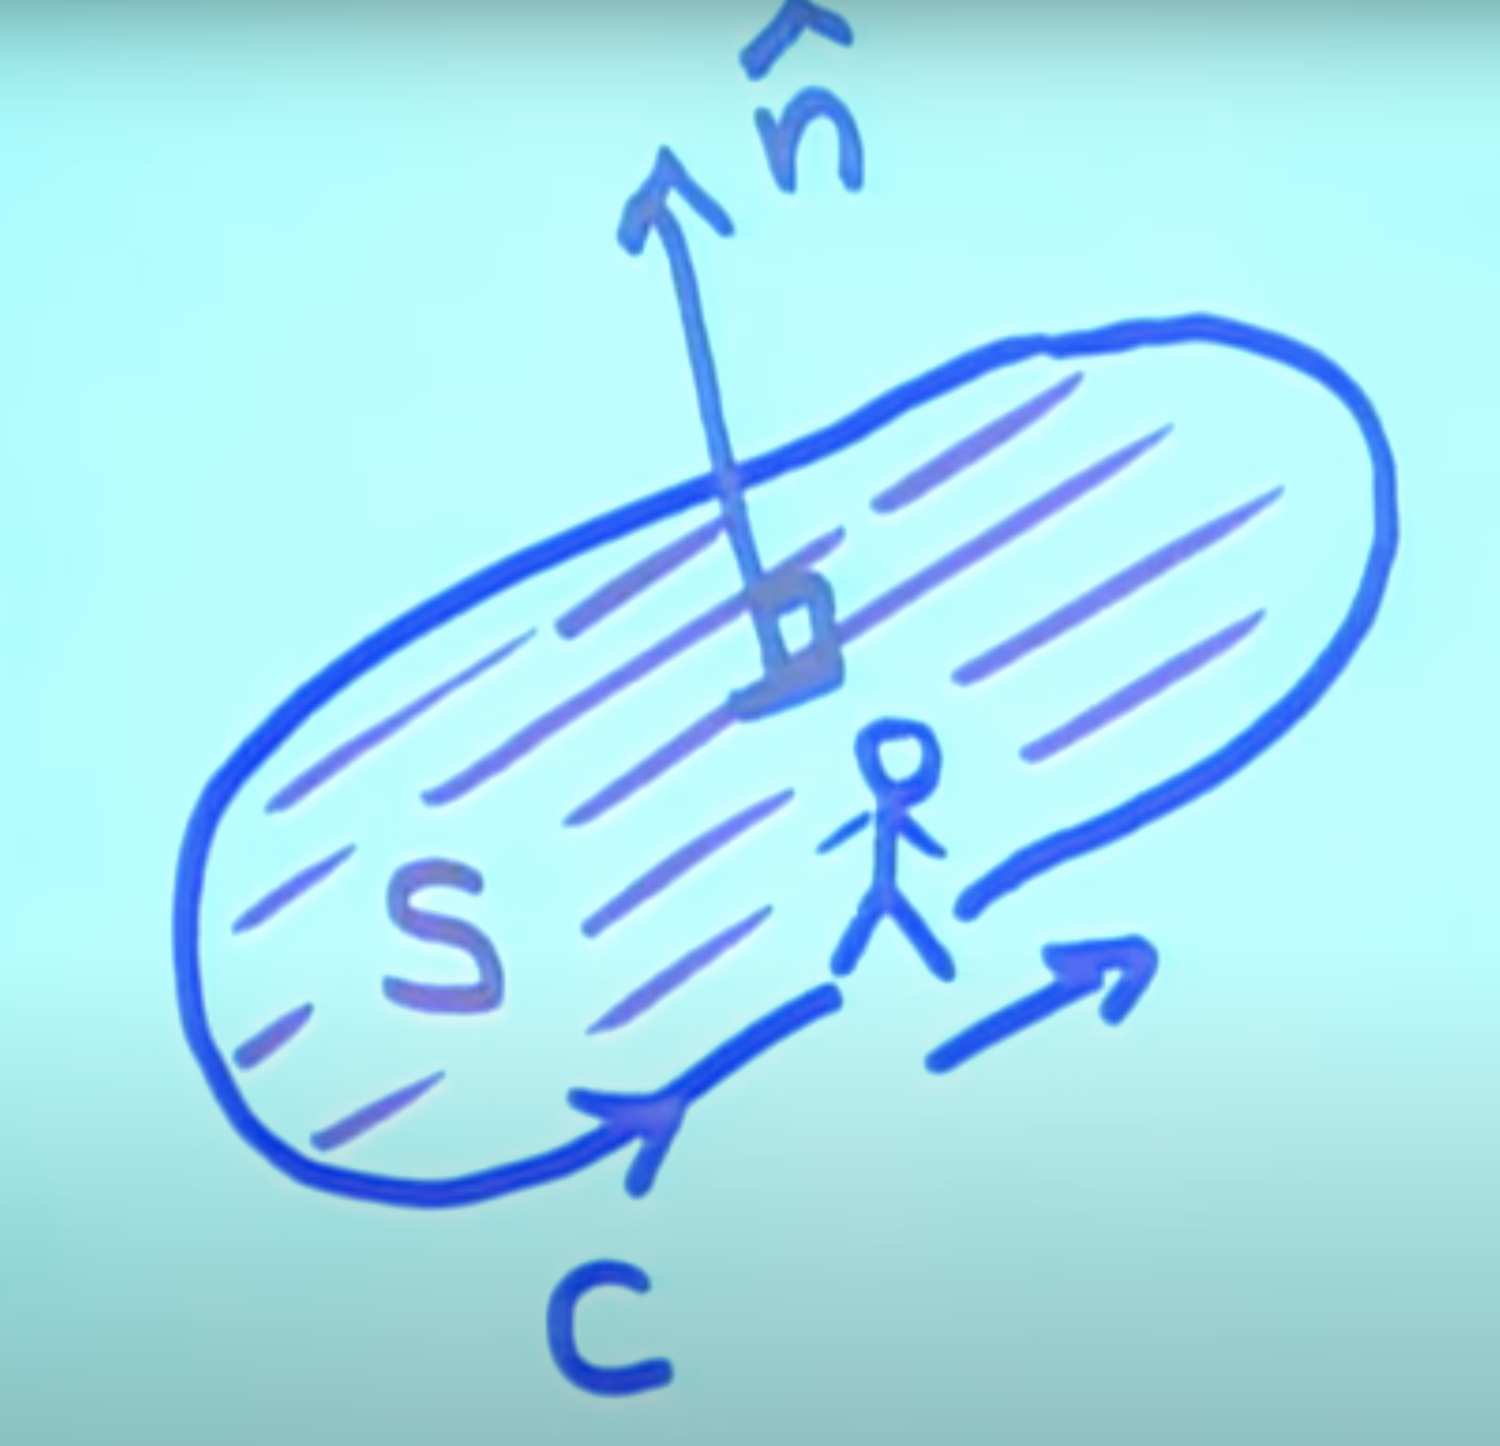
\includegraphics[scale=0.3]{./images/lecture_27_figure_1.png}
    \caption{Orianting Curve and Surface}
\end{figure}

Another way to do this is to use the right hand rule.
Point your thumg along the curve and point your index finger tangent the surface towards the interior of surface, 
then point your middle finger perpendicular to both and that will be the direction of the normal vector. 


\section{Comparing Stokes Theorem With Green's Theorem}

Let's say we have a closed curve lies in the $XY$-plane and goes in the counter clockwise direction.
And let $S$ be the surface in the $XY$-plane enclosed by $C$.
So if a vector field ${\bf F} = \left< P, Q, R \right>$ exists then 

$$ \oint_C {\bf F} \cdot d{\bf r} = \oint_C Pdx + Qdy $$

This is because we are in the $XY$-plane so $dz = 0$.
Now by Stokes' Theorem, 

$$ 
\oint_C {\bf F} \cdot d{\bf r} 
= \oint_C Pdx + Qdy 
= \iint_S (\nabla \times {\bf F}) \cdot \hat{n} dS 
$$

For our surface, the normal vector for our curve  will be $\hat{k}$. Now $(\nabla \times {\bf F}) \cdot \hat{k} = Q_x - P_y$
So, 

$$
\oint_C {\bf F} \cdot d{\bf r} 
= \oint_C Pdx + Qdy 
= \iint_S Q_x - P_y dS 
$$

This is exactly what Green's Theorem is. 
So Green's Theorem is just a special case of Stokes' Theorem in the $XY$-plane.
